\documentclass{standalone}
% analysis/style.tex — shared pgfplots preamble; % analysis/style.tex — shared pgfplots preamble; % analysis/style.tex — shared pgfplots preamble; \input{../style} from figures/
\usepackage[eulergreek]{sansmath}
\usepackage{pgfplots}
\usepackage{pgfplotstable}
\usepackage{xspace}

% Scheme-name macros — mirror the paper's meta/templates.tex so figure
% legends/titles/captions can write \plaintext / \sap / \emvp / \bntm /
% \tiptoe and render identically in both contexts. `\providecommand`
% lets the paper's templates.tex (loaded earlier) win when this file
% is in the paper as plots/pgfstyle.tex; in standalone artefact compiles
% these are the source of the macros.
\providecommand{\plaintext}{\textsc{Plaintext}\xspace}
\providecommand{\sap}{\textsc{SAP}\xspace}
\providecommand{\emvp}{\textsc{EMVP}\xspace}
\providecommand{\bntm}{\textsc{BNTM}\xspace}
\providecommand{\tiptoe}{\textsc{Tiptoe}\xspace}

\pgfplotsset{compat=newest}
\usepgfplotslibrary{units,colorbrewer,groupplots,fillbetween,statistics}
\usetikzlibrary{arrows.meta,backgrounds,calc,fit,shapes.geometric,positioning,patterns,shapes.misc}

% Bar charts request the colorbrewer Paired-12 cycle list directly via
% `cycle list/Paired-12` (loaded above by \usepgfplotslibrary{colorbrewer}).
% The library's `Paired-N` lists are full-colour, paper-quality, and live
% inside pgfplots so we don't ship a hand-rolled equivalent here.

\pgfplotsset{
  width=3.25in, height=2.5in,
  every axis/.append style={
    semithick,
    ymajorgrids=true,
    label style={font=\sffamily\small},
    title style={font=\sffamily\small},
  },
  % Line plots default to thick. `smooth` is NOT global — it is
  % opt-in per figure (added inside the axis options of figures 01,
  % 02, 04, 05, 06 that benefit from cubic interpolation). Putting
  % `smooth` in the global default fights pgfplots' `ybar` state
  % machine in figure 03 and `[only marks]` plots elsewhere; the
  % per-figure opt-in is cleaner than chasing local overrides.
  every axis plot/.append style={thick},
  legend style={
    draw=none,
    % Fully transparent legend container so overlap with plot title /
    % data points is visually obvious during figure tuning, rather
    % than silently masked. `fill=none` alone leaves an opaque white
    % rectangle on some pgfplots versions; pinning `fill opacity=0`
    % belt-and-braces guarantees see-through.
    fill=none,
    text opacity=1,
    anchor=south,
    at={(0.5,1)},
    font=\sffamily\small,
  },
  legend cell align=left,
  legend columns=-1,
  xtick align=outside,
  xtick pos=bottom,
  major tick length=1mm,
  tick label style={font=\sansmath\sffamily\small},
  every axis label={font=\sffamily\small},
  label style={font=\sffamily\small},
  {cycle list/Dark2},
  {cycle list/Set1},
  cycle list name=Dark2,
  cycle multiindex* list={
    Dark2\nextlist
    {solid,dashed,dotted,dashdotted,densely dashdotdotted}\nextlist
    mark list*\nextlist
  },
  /pgfplots/short line legend/.style={
    legend image code/.code={
      \draw[mark repeat=2,mark phase=2,##1]
        plot coordinates {(0cm,0cm)(0.2cm,0cm)(0.4cm,0cm)};
    }
  },
  /pgfplots/ybar legend/.style={
    /pgfplots/legend image code/.code={
      \draw[##1,/tikz/.cd,yshift=-0.25em](0cm,0cm) rectangle (4pt,6pt);
    },
  },
  /pgfplots/xbar legend/.style={
    /pgfplots/legend image code/.code={
      \draw[##1,/tikz/.cd,yshift=-0.25em](0cm,0cm) rectangle (4pt,6pt);
    },
  },
  select coords between index/.style 2 args={
    x filter/.code={
      \ifnum\coordindex<#1\def\pgfmathresult{}\fi
      \ifnum\coordindex>#2\def\pgfmathresult{}\fi
    }
  },
  discard if not/.style 2 args={
    x filter/.code={
      \edef\tempa{\thisrow{#1}}
      \edef\tempb{#2}
      \ifx\tempa\tempb
      \else
        \def\pgfmathresult{inf}
      \fi
    }
  },
}
 from figures/
\usepackage[eulergreek]{sansmath}
\usepackage{pgfplots}
\usepackage{pgfplotstable}
\usepackage{xspace}

% Scheme-name macros — mirror the paper's meta/templates.tex so figure
% legends/titles/captions can write \plaintext / \sap / \emvp / \bntm /
% \tiptoe and render identically in both contexts. `\providecommand`
% lets the paper's templates.tex (loaded earlier) win when this file
% is in the paper as plots/pgfstyle.tex; in standalone artefact compiles
% these are the source of the macros.
\providecommand{\plaintext}{\textsc{Plaintext}\xspace}
\providecommand{\sap}{\textsc{SAP}\xspace}
\providecommand{\emvp}{\textsc{EMVP}\xspace}
\providecommand{\bntm}{\textsc{BNTM}\xspace}
\providecommand{\tiptoe}{\textsc{Tiptoe}\xspace}

\pgfplotsset{compat=newest}
\usepgfplotslibrary{units,colorbrewer,groupplots,fillbetween,statistics}
\usetikzlibrary{arrows.meta,backgrounds,calc,fit,shapes.geometric,positioning,patterns,shapes.misc}

% Bar charts request the colorbrewer Paired-12 cycle list directly via
% `cycle list/Paired-12` (loaded above by \usepgfplotslibrary{colorbrewer}).
% The library's `Paired-N` lists are full-colour, paper-quality, and live
% inside pgfplots so we don't ship a hand-rolled equivalent here.

\pgfplotsset{
  width=3.25in, height=2.5in,
  every axis/.append style={
    semithick,
    ymajorgrids=true,
    label style={font=\sffamily\small},
    title style={font=\sffamily\small},
  },
  % Line plots default to thick. `smooth` is NOT global — it is
  % opt-in per figure (added inside the axis options of figures 01,
  % 02, 04, 05, 06 that benefit from cubic interpolation). Putting
  % `smooth` in the global default fights pgfplots' `ybar` state
  % machine in figure 03 and `[only marks]` plots elsewhere; the
  % per-figure opt-in is cleaner than chasing local overrides.
  every axis plot/.append style={thick},
  legend style={
    draw=none,
    % Fully transparent legend container so overlap with plot title /
    % data points is visually obvious during figure tuning, rather
    % than silently masked. `fill=none` alone leaves an opaque white
    % rectangle on some pgfplots versions; pinning `fill opacity=0`
    % belt-and-braces guarantees see-through.
    fill=none,
    text opacity=1,
    anchor=south,
    at={(0.5,1)},
    font=\sffamily\small,
  },
  legend cell align=left,
  legend columns=-1,
  xtick align=outside,
  xtick pos=bottom,
  major tick length=1mm,
  tick label style={font=\sansmath\sffamily\small},
  every axis label={font=\sffamily\small},
  label style={font=\sffamily\small},
  {cycle list/Dark2},
  {cycle list/Set1},
  cycle list name=Dark2,
  cycle multiindex* list={
    Dark2\nextlist
    {solid,dashed,dotted,dashdotted,densely dashdotdotted}\nextlist
    mark list*\nextlist
  },
  /pgfplots/short line legend/.style={
    legend image code/.code={
      \draw[mark repeat=2,mark phase=2,##1]
        plot coordinates {(0cm,0cm)(0.2cm,0cm)(0.4cm,0cm)};
    }
  },
  /pgfplots/ybar legend/.style={
    /pgfplots/legend image code/.code={
      \draw[##1,/tikz/.cd,yshift=-0.25em](0cm,0cm) rectangle (4pt,6pt);
    },
  },
  /pgfplots/xbar legend/.style={
    /pgfplots/legend image code/.code={
      \draw[##1,/tikz/.cd,yshift=-0.25em](0cm,0cm) rectangle (4pt,6pt);
    },
  },
  select coords between index/.style 2 args={
    x filter/.code={
      \ifnum\coordindex<#1\def\pgfmathresult{}\fi
      \ifnum\coordindex>#2\def\pgfmathresult{}\fi
    }
  },
  discard if not/.style 2 args={
    x filter/.code={
      \edef\tempa{\thisrow{#1}}
      \edef\tempb{#2}
      \ifx\tempa\tempb
      \else
        \def\pgfmathresult{inf}
      \fi
    }
  },
}
 from figures/
\usepackage[eulergreek]{sansmath}
\usepackage{pgfplots}
\usepackage{pgfplotstable}
\usepackage{xspace}

% Scheme-name macros — mirror the paper's meta/templates.tex so figure
% legends/titles/captions can write \plaintext / \sap / \emvp / \bntm /
% \tiptoe and render identically in both contexts. `\providecommand`
% lets the paper's templates.tex (loaded earlier) win when this file
% is in the paper as plots/pgfstyle.tex; in standalone artefact compiles
% these are the source of the macros.
\providecommand{\plaintext}{\textsc{Plaintext}\xspace}
\providecommand{\sap}{\textsc{SAP}\xspace}
\providecommand{\emvp}{\textsc{EMVP}\xspace}
\providecommand{\bntm}{\textsc{BNTM}\xspace}
\providecommand{\tiptoe}{\textsc{Tiptoe}\xspace}

\pgfplotsset{compat=newest}
\usepgfplotslibrary{units,colorbrewer,groupplots,fillbetween,statistics}
\usetikzlibrary{arrows.meta,backgrounds,calc,fit,shapes.geometric,positioning,patterns,shapes.misc}

% Bar charts request the colorbrewer Paired-12 cycle list directly via
% `cycle list/Paired-12` (loaded above by \usepgfplotslibrary{colorbrewer}).
% The library's `Paired-N` lists are full-colour, paper-quality, and live
% inside pgfplots so we don't ship a hand-rolled equivalent here.

\pgfplotsset{
  width=3.25in, height=2.5in,
  every axis/.append style={
    semithick,
    ymajorgrids=true,
    label style={font=\sffamily\small},
    title style={font=\sffamily\small},
  },
  % Line plots default to thick. `smooth` is NOT global — it is
  % opt-in per figure (added inside the axis options of figures 01,
  % 02, 04, 05, 06 that benefit from cubic interpolation). Putting
  % `smooth` in the global default fights pgfplots' `ybar` state
  % machine in figure 03 and `[only marks]` plots elsewhere; the
  % per-figure opt-in is cleaner than chasing local overrides.
  every axis plot/.append style={thick},
  legend style={
    draw=none,
    % Fully transparent legend container so overlap with plot title /
    % data points is visually obvious during figure tuning, rather
    % than silently masked. `fill=none` alone leaves an opaque white
    % rectangle on some pgfplots versions; pinning `fill opacity=0`
    % belt-and-braces guarantees see-through.
    fill=none,
    text opacity=1,
    anchor=south,
    at={(0.5,1)},
    font=\sffamily\small,
  },
  legend cell align=left,
  legend columns=-1,
  xtick align=outside,
  xtick pos=bottom,
  major tick length=1mm,
  tick label style={font=\sansmath\sffamily\small},
  every axis label={font=\sffamily\small},
  label style={font=\sffamily\small},
  {cycle list/Dark2},
  {cycle list/Set1},
  cycle list name=Dark2,
  cycle multiindex* list={
    Dark2\nextlist
    {solid,dashed,dotted,dashdotted,densely dashdotdotted}\nextlist
    mark list*\nextlist
  },
  /pgfplots/short line legend/.style={
    legend image code/.code={
      \draw[mark repeat=2,mark phase=2,##1]
        plot coordinates {(0cm,0cm)(0.2cm,0cm)(0.4cm,0cm)};
    }
  },
  /pgfplots/ybar legend/.style={
    /pgfplots/legend image code/.code={
      \draw[##1,/tikz/.cd,yshift=-0.25em](0cm,0cm) rectangle (4pt,6pt);
    },
  },
  /pgfplots/xbar legend/.style={
    /pgfplots/legend image code/.code={
      \draw[##1,/tikz/.cd,yshift=-0.25em](0cm,0cm) rectangle (4pt,6pt);
    },
  },
  select coords between index/.style 2 args={
    x filter/.code={
      \ifnum\coordindex<#1\def\pgfmathresult{}\fi
      \ifnum\coordindex>#2\def\pgfmathresult{}\fi
    }
  },
  discard if not/.style 2 args={
    x filter/.code={
      \edef\tempa{\thisrow{#1}}
      \edef\tempb{#2}
      \ifx\tempa\tempb
      \else
        \def\pgfmathresult{inf}
      \fi
    }
  },
}

\providecommand{\datadir}{../data}
\begin{document}
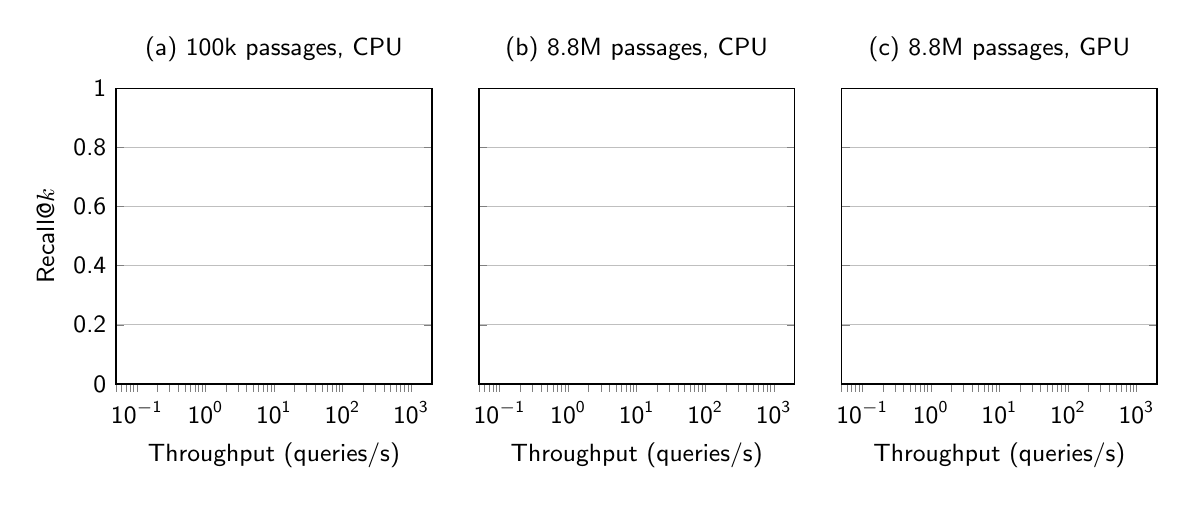
\begin{tikzpicture}
  % Per-scheme colour + mark + line-style bindings shared across all
  % three panels. The explicit `solid` is load-bearing: style.tex sets
  % `cycle multiindex* list={Dark2, {solid,dashed,dotted,...}, marks}`,
  % so without an override the IVF schemes would inherit a different
  % line dash style in every panel (panel A used 5 plots and tripped
  % through solid/dashed/dotted/dashdotted/dashdotdotted; panels B/C
  % reset to solid because \nextgroupplot rewinds the cycle).
  \pgfplotsset{
    plaintext/.style={color=Set1-A, mark=*,        solid},
    sapivf/.style   ={color=Set1-B, mark=square*,  solid},
    emvpivf/.style  ={color=Set1-C, mark=triangle*,solid},
    bnivf/.style    ={color=Set1-D, mark=diamond*, solid},
    tiptoe/.style   ={color=Set1-E, mark=x,        densely dotted},
  }
  \begin{groupplot}[
    group style={
      group size=3 by 1,
      horizontal sep=0.6cm,
      ylabels at=edge left,
      yticklabels at=edge left,
    },
    width=2.2in, height=2.1in,
    xlabel={Throughput (queries/s)},
    ylabel={Recall@$k$},
    xmode=log,
    % Shared x range so the three panels read as a like-for-like
    % comparison; bounds chosen to bracket every series across the
    % three panels (low end driven by \emvp+IVF / \bntm+IVF at 8.8M;
    % high end driven by \plaintext+IVF / \sap+IVF at 100k).
    xmin=0.05, xmax=2000,
    ymin=0, ymax=1,
    every axis plot/.append style={
      smooth,
      error bars/x dir=both,
      error bars/x explicit,
    },
    title style={font=\sffamily\small},
  ]
    % ── Panel A — 100k passages, CPU (sacs006) ──────────────────────
    % `legend to name` lives on Panel A only: in groupplot's shared
    % options it fires per `\nextgroupplot`, and panels B / C
    % (intentionally entry-less) would overwrite the captured legend
    % with an empty one.
    \nextgroupplot[
      title={(a) 100k passages, CPU},
      legend to name=fig02legend,
      legend columns=-1,
      legend style={font=\sffamily\small},
    ]
    \IfFileExists{\datadir/recall-throughput-100k-cpu-plaintext.tsv}{
      \addplot+[plaintext] table[col sep=tab, x=qps, x error=qps_rep_ci95, y=recall_mean]
        {\datadir/recall-throughput-100k-cpu-plaintext.tsv};
      \addlegendentry{\plaintext+IVF}
    }{}
    \IfFileExists{\datadir/recall-throughput-100k-cpu-sap-ivf-nprobe.tsv}{
      \addplot+[sapivf] table[col sep=tab, x=qps, x error=qps_rep_ci95, y=recall_mean]
        {\datadir/recall-throughput-100k-cpu-sap-ivf-nprobe.tsv};
      \addlegendentry{\sap+IVF}
    }{}
    \IfFileExists{\datadir/recall-throughput-100k-cpu-emvp-ivf-nprobe.tsv}{
      \addplot+[emvpivf] table[col sep=tab, x=qps, x error=qps_rep_ci95, y=recall_mean]
        {\datadir/recall-throughput-100k-cpu-emvp-ivf-nprobe.tsv};
      \addlegendentry{\emvp+IVF}
    }{}
    \IfFileExists{\datadir/recall-throughput-100k-cpu-bntm-ivf-nprobe.tsv}{
      \addplot+[bnivf] table[col sep=tab, x=qps, x error=qps_rep_ci95, y=recall_mean]
        {\datadir/recall-throughput-100k-cpu-bntm-ivf-nprobe.tsv};
      \addlegendentry{\bntm+IVF}
    }{}
    \IfFileExists{\datadir/recall-throughput-100k-cpu-tiptoe.tsv}{
      \addplot+[tiptoe] table[col sep=tab, x=qps, x error=qps_rep_ci95, y=recall_mean]
        {\datadir/recall-throughput-100k-cpu-tiptoe.tsv};
      \addlegendentry{\tiptoe}
    }{}

    % ── Panel B — 8.8M passages, CPU ────────────────────────────────
    % Only IVF schemes have 8.8M data: flat scorers and \tiptoe are
    % off the chart for cost reasons. `forget plot` suppresses the
    % duplicate legend entries (the panel A entries are canonical).
    \nextgroupplot[title={(b) 8.8M passages, CPU}]
    \IfFileExists{\datadir/recall-throughput-8m-cpu-plaintext.tsv}{
      \addplot+[plaintext, forget plot] table[col sep=tab, x=qps, x error=qps_rep_ci95, y=recall_mean]
        {\datadir/recall-throughput-8m-cpu-plaintext.tsv};
    }{}
    \IfFileExists{\datadir/recall-throughput-8m-cpu-sap-ivf-nprobe.tsv}{
      \addplot+[sapivf, forget plot] table[col sep=tab, x=qps, x error=qps_rep_ci95, y=recall_mean]
        {\datadir/recall-throughput-8m-cpu-sap-ivf-nprobe.tsv};
    }{}
    \IfFileExists{\datadir/recall-throughput-8m-cpu-emvp-ivf-nprobe.tsv}{
      \addplot+[emvpivf, forget plot] table[col sep=tab, x=qps, x error=qps_rep_ci95, y=recall_mean]
        {\datadir/recall-throughput-8m-cpu-emvp-ivf-nprobe.tsv};
    }{}
    \IfFileExists{\datadir/recall-throughput-8m-cpu-bntm-ivf-nprobe.tsv}{
      \addplot+[bnivf, forget plot] table[col sep=tab, x=qps, x error=qps_rep_ci95, y=recall_mean]
        {\datadir/recall-throughput-8m-cpu-bntm-ivf-nprobe.tsv};
    }{}

    % ── Panel C — 8.8M passages, GPU ────────────────────────────────
    \nextgroupplot[title={(c) 8.8M passages, GPU}]
    \IfFileExists{\datadir/recall-throughput-8m-gpu-plaintext.tsv}{
      \addplot+[plaintext, forget plot] table[col sep=tab, x=qps, x error=qps_rep_ci95, y=recall_mean]
        {\datadir/recall-throughput-8m-gpu-plaintext.tsv};
    }{}
    \IfFileExists{\datadir/recall-throughput-8m-gpu-sap-ivf-nprobe.tsv}{
      \addplot+[sapivf, forget plot] table[col sep=tab, x=qps, x error=qps_rep_ci95, y=recall_mean]
        {\datadir/recall-throughput-8m-gpu-sap-ivf-nprobe.tsv};
    }{}
    \IfFileExists{\datadir/recall-throughput-8m-gpu-emvp-ivf-nprobe.tsv}{
      \addplot+[emvpivf, forget plot] table[col sep=tab, x=qps, x error=qps_rep_ci95, y=recall_mean]
        {\datadir/recall-throughput-8m-gpu-emvp-ivf-nprobe.tsv};
    }{}
    \IfFileExists{\datadir/recall-throughput-8m-gpu-bntm-ivf-nprobe.tsv}{
      \addplot+[bnivf, forget plot] table[col sep=tab, x=qps, x error=qps_rep_ci95, y=recall_mean]
        {\datadir/recall-throughput-8m-gpu-bntm-ivf-nprobe.tsv};
    }{}
  \end{groupplot}
  % Shared legend, centred above the midpoint of the three panels.
  % `\pgfplotslegendfromname` renders the captured legend in one pass,
  % unlike `\ref{fig02legend}` which forward-references a `\label` —
  % the latter fails under tikzexternalize (single-pass subprocess
  % can't resolve a label written in the same pass). yshift clears
  % each panel's title text.
  \node[anchor=south, inner sep=0pt, yshift=20pt]
    at (group c2r1.north) {\pgfplotslegendfromname{fig02legend}};
\end{tikzpicture}
\end{document}
